\documentclass[twoside]{book}

% Packages required by doxygen
\usepackage{fixltx2e}
\usepackage{calc}
\usepackage{doxygen}
\usepackage[export]{adjustbox} % also loads graphicx
\usepackage{graphicx}
\usepackage[utf8]{inputenc}
\usepackage{makeidx}
\usepackage{multicol}
\usepackage{multirow}
\PassOptionsToPackage{warn}{textcomp}
\usepackage{textcomp}
\usepackage[nointegrals]{wasysym}
\usepackage[table]{xcolor}

% Font selection
\usepackage[T1]{fontenc}
\usepackage[scaled=.90]{helvet}
\usepackage{courier}
\usepackage{amssymb}
\usepackage{sectsty}
\renewcommand{\familydefault}{\sfdefault}
\allsectionsfont{%
  \fontseries{bc}\selectfont%
  \color{darkgray}%
}
\renewcommand{\DoxyLabelFont}{%
  \fontseries{bc}\selectfont%
  \color{darkgray}%
}
\newcommand{\+}{\discretionary{\mbox{\scriptsize$\hookleftarrow$}}{}{}}

% Page & text layout
\usepackage{geometry}
\geometry{%
  a4paper,%
  top=2.5cm,%
  bottom=2.5cm,%
  left=2.5cm,%
  right=2.5cm%
}
\tolerance=750
\hfuzz=15pt
\hbadness=750
\setlength{\emergencystretch}{15pt}
\setlength{\parindent}{0cm}
\setlength{\parskip}{3ex plus 2ex minus 2ex}
\makeatletter
\renewcommand{\paragraph}{%
  \@startsection{paragraph}{4}{0ex}{-1.0ex}{1.0ex}{%
    \normalfont\normalsize\bfseries\SS@parafont%
  }%
}
\renewcommand{\subparagraph}{%
  \@startsection{subparagraph}{5}{0ex}{-1.0ex}{1.0ex}{%
    \normalfont\normalsize\bfseries\SS@subparafont%
  }%
}
\makeatother

% Headers & footers
\usepackage{fancyhdr}
\pagestyle{fancyplain}
\fancyhead[LE]{\fancyplain{}{\bfseries\thepage}}
\fancyhead[CE]{\fancyplain{}{}}
\fancyhead[RE]{\fancyplain{}{\bfseries\leftmark}}
\fancyhead[LO]{\fancyplain{}{\bfseries\rightmark}}
\fancyhead[CO]{\fancyplain{}{}}
\fancyhead[RO]{\fancyplain{}{\bfseries\thepage}}
\fancyfoot[LE]{\fancyplain{}{}}
\fancyfoot[CE]{\fancyplain{}{}}
\fancyfoot[RE]{\fancyplain{}{\bfseries\scriptsize Generated by Doxygen }}
\fancyfoot[LO]{\fancyplain{}{\bfseries\scriptsize Generated by Doxygen }}
\fancyfoot[CO]{\fancyplain{}{}}
\fancyfoot[RO]{\fancyplain{}{}}
\renewcommand{\footrulewidth}{0.4pt}
\renewcommand{\chaptermark}[1]{%
  \markboth{#1}{}%
}
\renewcommand{\sectionmark}[1]{%
  \markright{\thesection\ #1}%
}

% Indices & bibliography
\usepackage{natbib}
\usepackage[titles]{tocloft}
\setcounter{tocdepth}{3}
\setcounter{secnumdepth}{5}
\makeindex

% Hyperlinks (required, but should be loaded last)
\usepackage{ifpdf}
\ifpdf
  \usepackage[pdftex,pagebackref=true]{hyperref}
\else
  \usepackage[ps2pdf,pagebackref=true]{hyperref}
\fi
\hypersetup{%
  colorlinks=true,%
  linkcolor=blue,%
  citecolor=blue,%
  unicode%
}

% Custom commands
\newcommand{\clearemptydoublepage}{%
  \newpage{\pagestyle{empty}\cleardoublepage}%
}

\usepackage{caption}
\captionsetup{labelsep=space,justification=centering,font={bf},singlelinecheck=off,skip=4pt,position=top}

%===== C O N T E N T S =====

\begin{document}

% Titlepage & ToC
\hypersetup{pageanchor=false,
             bookmarksnumbered=true,
             pdfencoding=unicode
            }
\pagenumbering{alph}
\begin{titlepage}
\vspace*{7cm}
\begin{center}%
{\Large Linked List }\\
\vspace*{1cm}
{\large Generated by Doxygen 1.8.13}\\
\end{center}
\end{titlepage}
\clearemptydoublepage
\pagenumbering{roman}
\tableofcontents
\clearemptydoublepage
\pagenumbering{arabic}
\hypersetup{pageanchor=true}

%--- Begin generated contents ---
\chapter{Class Index}
\section{Class List}
Here are the classes, structs, unions and interfaces with brief descriptions\+:\begin{DoxyCompactList}
\item\contentsline{section}{\hyperlink{classCRAZYFISH_1_1LinkedList}{C\+R\+A\+Z\+Y\+F\+I\+S\+H\+::\+Linked\+List$<$ T\+Y\+P\+E $>$} }{\pageref{classCRAZYFISH_1_1LinkedList}}{}
\item\contentsline{section}{\hyperlink{classCRAZYFISH_1_1LinkedList_1_1Node}{C\+R\+A\+Z\+Y\+F\+I\+S\+H\+::\+Linked\+List$<$ T\+Y\+P\+E $>$\+::\+Node} }{\pageref{classCRAZYFISH_1_1LinkedList_1_1Node}}{}
\end{DoxyCompactList}

\chapter{File Index}
\section{File List}
Here is a list of all documented files with brief descriptions\+:\begin{DoxyCompactList}
\item\contentsline{section}{\hyperlink{LinkedList_8h}{Linked\+List.\+h} \\*An implementation of the dynamic A\+DT List. This is a demo for teaching, N\+OT recommended for any practical job }{\pageref{LinkedList_8h}}{}
\item\contentsline{section}{{\bfseries Linked\+List.\+templates.\+h} }{\pageref{LinkedList_8templates_8h}}{}
\end{DoxyCompactList}

\chapter{Class Documentation}
\hypertarget{classCRAZYFISH_1_1LinkedList}{}\section{C\+R\+A\+Z\+Y\+F\+I\+SH\+:\+:Linked\+List$<$ T\+Y\+PE $>$ Class Template Reference}
\label{classCRAZYFISH_1_1LinkedList}\index{C\+R\+A\+Z\+Y\+F\+I\+S\+H\+::\+Linked\+List$<$ T\+Y\+P\+E $>$@{C\+R\+A\+Z\+Y\+F\+I\+S\+H\+::\+Linked\+List$<$ T\+Y\+P\+E $>$}}


{\ttfamily \#include $<$Linked\+List.\+h$>$}



Collaboration diagram for C\+R\+A\+Z\+Y\+F\+I\+SH\+:\+:Linked\+List$<$ T\+Y\+PE $>$\+:\nopagebreak
\begin{figure}[H]
\begin{center}
\leavevmode
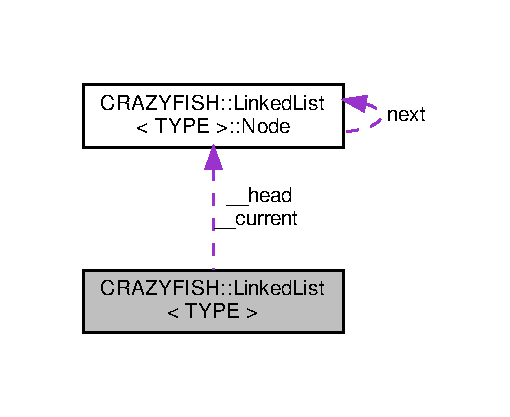
\includegraphics[width=245pt]{classCRAZYFISH_1_1LinkedList__coll__graph}
\end{center}
\end{figure}
\subsection*{Classes}
\begin{DoxyCompactItemize}
\item 
class \hyperlink{classCRAZYFISH_1_1LinkedList_1_1Node}{Node}
\end{DoxyCompactItemize}
\subsection*{Public Member Functions}
\begin{DoxyCompactItemize}
\item 
\hyperlink{classCRAZYFISH_1_1LinkedList_a8cfb7db8375d42e804107bed6ee300d8}{Linked\+List} ()
\item 
\hyperlink{classCRAZYFISH_1_1LinkedList_a97ff37e22764e437dfeff71c686cfbd0}{Linked\+List} (\hyperlink{classCRAZYFISH_1_1LinkedList_1_1Node}{Node} \&\+\_\+new)
\item 
\hyperlink{classCRAZYFISH_1_1LinkedList_a5d084245dc02a983ba9645c80fc14cea}{Linked\+List} (T\+Y\+PE \&\+\_\+val)
\item 
\hyperlink{classCRAZYFISH_1_1LinkedList_a6e2311f3cc0ef21d731e0f17a005eca0}{$\sim$\+Linked\+List} ()
\item 
int \hyperlink{classCRAZYFISH_1_1LinkedList_aef8407ee5167b26ed5a5707fc2886fb8}{print\+Linked\+List} ()
\item 
T\+Y\+PE $\ast$ \hyperlink{classCRAZYFISH_1_1LinkedList_a9ec77e618ea899c8458824a2a10066de}{find} (T\+Y\+PE \+\_\+d)
\item 
int \hyperlink{classCRAZYFISH_1_1LinkedList_a114e00935149d4c6fb68cc4654a4904c}{insert} (\hyperlink{classCRAZYFISH_1_1LinkedList_1_1Node}{Node} \&\+\_\+new)
\item 
int \hyperlink{classCRAZYFISH_1_1LinkedList_a431acbe0a25d8e3d56994fcd427d21d7}{insert} (T\+Y\+PE \&\+\_\+val)
\item 
int \hyperlink{classCRAZYFISH_1_1LinkedList_aed4f2193935fb362eae3d47bb789edee}{del} ()
\end{DoxyCompactItemize}
\subsection*{Private Attributes}
\begin{DoxyCompactItemize}
\item 
\hyperlink{classCRAZYFISH_1_1LinkedList_1_1Node}{Node} $\ast$ \hyperlink{classCRAZYFISH_1_1LinkedList_a1439d0f5f10624ffd090cdec5430390d}{\+\_\+\+\_\+head}
\item 
\hyperlink{classCRAZYFISH_1_1LinkedList_1_1Node}{Node} $\ast$ \hyperlink{classCRAZYFISH_1_1LinkedList_aa964652536c838dbbe87900de5f8816e}{\+\_\+\+\_\+current}
\item 
int \hyperlink{classCRAZYFISH_1_1LinkedList_afe0f4aa3de15119600fd14c4a6ed3fc1}{\+\_\+\+\_\+length}
\end{DoxyCompactItemize}
\subsection*{Friends}
\begin{DoxyCompactItemize}
\item 
std\+::ostream \& \hyperlink{classCRAZYFISH_1_1LinkedList_a77f02bc38eca13d0374fd4b50b1b17a1}{operator$<$$<$} (std\+::ostream \&, const \hyperlink{classCRAZYFISH_1_1LinkedList}{Linked\+List}$<$ T\+Y\+PE $>$ \&)
\end{DoxyCompactItemize}


\subsection{Detailed Description}
\subsubsection*{template$<$class T\+Y\+PE$>$\newline
class C\+R\+A\+Z\+Y\+F\+I\+S\+H\+::\+Linked\+List$<$ T\+Y\+P\+E $>$}

Using standard array in C++ to implement List A\+DT. T\+Y\+PE can be char, int, long, double or long double. 

\subsection{Constructor \& Destructor Documentation}
\mbox{\Hypertarget{classCRAZYFISH_1_1LinkedList_a8cfb7db8375d42e804107bed6ee300d8}\label{classCRAZYFISH_1_1LinkedList_a8cfb7db8375d42e804107bed6ee300d8}} 
\index{C\+R\+A\+Z\+Y\+F\+I\+S\+H\+::\+Linked\+List@{C\+R\+A\+Z\+Y\+F\+I\+S\+H\+::\+Linked\+List}!Linked\+List@{Linked\+List}}
\index{Linked\+List@{Linked\+List}!C\+R\+A\+Z\+Y\+F\+I\+S\+H\+::\+Linked\+List@{C\+R\+A\+Z\+Y\+F\+I\+S\+H\+::\+Linked\+List}}
\subsubsection{\texorpdfstring{Linked\+List()}{LinkedList()}\hspace{0.1cm}{\footnotesize\ttfamily [1/3]}}
{\footnotesize\ttfamily template$<$class T\+Y\+PE$>$ \\
\hyperlink{classCRAZYFISH_1_1LinkedList}{C\+R\+A\+Z\+Y\+F\+I\+S\+H\+::\+Linked\+List}$<$ T\+Y\+PE $>$\+::\hyperlink{classCRAZYFISH_1_1LinkedList}{Linked\+List} (\begin{DoxyParamCaption}{ }\end{DoxyParamCaption})\hspace{0.3cm}{\ttfamily [inline]}}

The default constructor. Build an empty List. \mbox{\Hypertarget{classCRAZYFISH_1_1LinkedList_a97ff37e22764e437dfeff71c686cfbd0}\label{classCRAZYFISH_1_1LinkedList_a97ff37e22764e437dfeff71c686cfbd0}} 
\index{C\+R\+A\+Z\+Y\+F\+I\+S\+H\+::\+Linked\+List@{C\+R\+A\+Z\+Y\+F\+I\+S\+H\+::\+Linked\+List}!Linked\+List@{Linked\+List}}
\index{Linked\+List@{Linked\+List}!C\+R\+A\+Z\+Y\+F\+I\+S\+H\+::\+Linked\+List@{C\+R\+A\+Z\+Y\+F\+I\+S\+H\+::\+Linked\+List}}
\subsubsection{\texorpdfstring{Linked\+List()}{LinkedList()}\hspace{0.1cm}{\footnotesize\ttfamily [2/3]}}
{\footnotesize\ttfamily template$<$class T\+Y\+PE $>$ \\
\hyperlink{classCRAZYFISH_1_1LinkedList}{C\+R\+A\+Z\+Y\+F\+I\+S\+H\+::\+Linked\+List}$<$ T\+Y\+PE $>$\+::\hyperlink{classCRAZYFISH_1_1LinkedList}{Linked\+List} (\begin{DoxyParamCaption}\item[{\hyperlink{classCRAZYFISH_1_1LinkedList_1_1Node}{Node} \&}]{\+\_\+new }\end{DoxyParamCaption})}

Constructor, build a List with the first element is \+\_\+new.


\begin{DoxyParams}{Parameters}
{\em \+\_\+new} & An assigned node. \\
\hline
\end{DoxyParams}
\mbox{\Hypertarget{classCRAZYFISH_1_1LinkedList_a5d084245dc02a983ba9645c80fc14cea}\label{classCRAZYFISH_1_1LinkedList_a5d084245dc02a983ba9645c80fc14cea}} 
\index{C\+R\+A\+Z\+Y\+F\+I\+S\+H\+::\+Linked\+List@{C\+R\+A\+Z\+Y\+F\+I\+S\+H\+::\+Linked\+List}!Linked\+List@{Linked\+List}}
\index{Linked\+List@{Linked\+List}!C\+R\+A\+Z\+Y\+F\+I\+S\+H\+::\+Linked\+List@{C\+R\+A\+Z\+Y\+F\+I\+S\+H\+::\+Linked\+List}}
\subsubsection{\texorpdfstring{Linked\+List()}{LinkedList()}\hspace{0.1cm}{\footnotesize\ttfamily [3/3]}}
{\footnotesize\ttfamily template$<$class T\+Y\+PE $>$ \\
\hyperlink{classCRAZYFISH_1_1LinkedList}{C\+R\+A\+Z\+Y\+F\+I\+S\+H\+::\+Linked\+List}$<$ T\+Y\+PE $>$\+::\hyperlink{classCRAZYFISH_1_1LinkedList}{Linked\+List} (\begin{DoxyParamCaption}\item[{T\+Y\+PE \&}]{\+\_\+val }\end{DoxyParamCaption})}

Constructor, build a List with the value of the first element is \+\_\+val.


\begin{DoxyParams}{Parameters}
{\em \+\_\+new} & An assigned node. \\
\hline
\end{DoxyParams}
\mbox{\Hypertarget{classCRAZYFISH_1_1LinkedList_a6e2311f3cc0ef21d731e0f17a005eca0}\label{classCRAZYFISH_1_1LinkedList_a6e2311f3cc0ef21d731e0f17a005eca0}} 
\index{C\+R\+A\+Z\+Y\+F\+I\+S\+H\+::\+Linked\+List@{C\+R\+A\+Z\+Y\+F\+I\+S\+H\+::\+Linked\+List}!````~Linked\+List@{$\sim$\+Linked\+List}}
\index{````~Linked\+List@{$\sim$\+Linked\+List}!C\+R\+A\+Z\+Y\+F\+I\+S\+H\+::\+Linked\+List@{C\+R\+A\+Z\+Y\+F\+I\+S\+H\+::\+Linked\+List}}
\subsubsection{\texorpdfstring{$\sim$\+Linked\+List()}{~LinkedList()}}
{\footnotesize\ttfamily template$<$class T\+Y\+PE$>$ \\
\hyperlink{classCRAZYFISH_1_1LinkedList}{C\+R\+A\+Z\+Y\+F\+I\+S\+H\+::\+Linked\+List}$<$ T\+Y\+PE $>$\+::$\sim$\hyperlink{classCRAZYFISH_1_1LinkedList}{Linked\+List} (\begin{DoxyParamCaption}{ }\end{DoxyParamCaption})}

Default destructor. 

\subsection{Member Function Documentation}
\mbox{\Hypertarget{classCRAZYFISH_1_1LinkedList_aed4f2193935fb362eae3d47bb789edee}\label{classCRAZYFISH_1_1LinkedList_aed4f2193935fb362eae3d47bb789edee}} 
\index{C\+R\+A\+Z\+Y\+F\+I\+S\+H\+::\+Linked\+List@{C\+R\+A\+Z\+Y\+F\+I\+S\+H\+::\+Linked\+List}!del@{del}}
\index{del@{del}!C\+R\+A\+Z\+Y\+F\+I\+S\+H\+::\+Linked\+List@{C\+R\+A\+Z\+Y\+F\+I\+S\+H\+::\+Linked\+List}}
\subsubsection{\texorpdfstring{del()}{del()}}
{\footnotesize\ttfamily template$<$class T\+Y\+PE $>$ \\
int \hyperlink{classCRAZYFISH_1_1LinkedList}{C\+R\+A\+Z\+Y\+F\+I\+S\+H\+::\+Linked\+List}$<$ T\+Y\+PE $>$\+::del (\begin{DoxyParamCaption}{ }\end{DoxyParamCaption})}

Delete the node A\+F\+T\+ER the current pointer. If the current one is head, then delete the first one if it exists or do nothing if the List is empty. Can not use name delete because it\textquotesingle{}s a key word.

\begin{DoxyReturn}{Returns}
0 for OK -\/1 for else. 
\end{DoxyReturn}
\mbox{\Hypertarget{classCRAZYFISH_1_1LinkedList_a9ec77e618ea899c8458824a2a10066de}\label{classCRAZYFISH_1_1LinkedList_a9ec77e618ea899c8458824a2a10066de}} 
\index{C\+R\+A\+Z\+Y\+F\+I\+S\+H\+::\+Linked\+List@{C\+R\+A\+Z\+Y\+F\+I\+S\+H\+::\+Linked\+List}!find@{find}}
\index{find@{find}!C\+R\+A\+Z\+Y\+F\+I\+S\+H\+::\+Linked\+List@{C\+R\+A\+Z\+Y\+F\+I\+S\+H\+::\+Linked\+List}}
\subsubsection{\texorpdfstring{find()}{find()}}
{\footnotesize\ttfamily template$<$class T\+Y\+PE $>$ \\
T\+Y\+PE $\ast$ \hyperlink{classCRAZYFISH_1_1LinkedList}{C\+R\+A\+Z\+Y\+F\+I\+S\+H\+::\+Linked\+List}$<$ T\+Y\+PE $>$\+::find (\begin{DoxyParamCaption}\item[{T\+Y\+PE}]{\+\_\+d }\end{DoxyParamCaption})}

Find if the List contains value \+\_\+d.


\begin{DoxyParams}{Parameters}
{\em \+\_\+d} & The value to find.\\
\hline
\end{DoxyParams}
\begin{DoxyReturn}{Returns}
The address of the first node with value \+\_\+d if found, otherwise N\+U\+LL. 
\end{DoxyReturn}
\mbox{\Hypertarget{classCRAZYFISH_1_1LinkedList_a114e00935149d4c6fb68cc4654a4904c}\label{classCRAZYFISH_1_1LinkedList_a114e00935149d4c6fb68cc4654a4904c}} 
\index{C\+R\+A\+Z\+Y\+F\+I\+S\+H\+::\+Linked\+List@{C\+R\+A\+Z\+Y\+F\+I\+S\+H\+::\+Linked\+List}!insert@{insert}}
\index{insert@{insert}!C\+R\+A\+Z\+Y\+F\+I\+S\+H\+::\+Linked\+List@{C\+R\+A\+Z\+Y\+F\+I\+S\+H\+::\+Linked\+List}}
\subsubsection{\texorpdfstring{insert()}{insert()}\hspace{0.1cm}{\footnotesize\ttfamily [1/2]}}
{\footnotesize\ttfamily template$<$class T\+Y\+PE $>$ \\
int \hyperlink{classCRAZYFISH_1_1LinkedList}{C\+R\+A\+Z\+Y\+F\+I\+S\+H\+::\+Linked\+List}$<$ T\+Y\+PE $>$\+::insert (\begin{DoxyParamCaption}\item[{\hyperlink{classCRAZYFISH_1_1LinkedList_1_1Node}{Node} \&}]{\+\_\+new }\end{DoxyParamCaption})}

Insert a new node after the current pointer. If the List is empty, then add it as the first node.


\begin{DoxyParams}{Parameters}
{\em \+\_\+new} & New node.\\
\hline
\end{DoxyParams}
\begin{DoxyReturn}{Returns}
0 for OK -\/1 for else. 
\end{DoxyReturn}
\mbox{\Hypertarget{classCRAZYFISH_1_1LinkedList_a431acbe0a25d8e3d56994fcd427d21d7}\label{classCRAZYFISH_1_1LinkedList_a431acbe0a25d8e3d56994fcd427d21d7}} 
\index{C\+R\+A\+Z\+Y\+F\+I\+S\+H\+::\+Linked\+List@{C\+R\+A\+Z\+Y\+F\+I\+S\+H\+::\+Linked\+List}!insert@{insert}}
\index{insert@{insert}!C\+R\+A\+Z\+Y\+F\+I\+S\+H\+::\+Linked\+List@{C\+R\+A\+Z\+Y\+F\+I\+S\+H\+::\+Linked\+List}}
\subsubsection{\texorpdfstring{insert()}{insert()}\hspace{0.1cm}{\footnotesize\ttfamily [2/2]}}
{\footnotesize\ttfamily template$<$class T\+Y\+PE$>$ \\
int \hyperlink{classCRAZYFISH_1_1LinkedList}{C\+R\+A\+Z\+Y\+F\+I\+S\+H\+::\+Linked\+List}$<$ T\+Y\+PE $>$\+::insert (\begin{DoxyParamCaption}\item[{T\+Y\+PE \&}]{\+\_\+val }\end{DoxyParamCaption})}

Insert a new node after the current pointer. If the List is empty, then add it as the first node.


\begin{DoxyParams}{Parameters}
{\em \+\_\+val} & The value in the new node.\\
\hline
\end{DoxyParams}
\begin{DoxyReturn}{Returns}
0 for OK -\/1 for else. 
\end{DoxyReturn}
\mbox{\Hypertarget{classCRAZYFISH_1_1LinkedList_aef8407ee5167b26ed5a5707fc2886fb8}\label{classCRAZYFISH_1_1LinkedList_aef8407ee5167b26ed5a5707fc2886fb8}} 
\index{C\+R\+A\+Z\+Y\+F\+I\+S\+H\+::\+Linked\+List@{C\+R\+A\+Z\+Y\+F\+I\+S\+H\+::\+Linked\+List}!print\+Linked\+List@{print\+Linked\+List}}
\index{print\+Linked\+List@{print\+Linked\+List}!C\+R\+A\+Z\+Y\+F\+I\+S\+H\+::\+Linked\+List@{C\+R\+A\+Z\+Y\+F\+I\+S\+H\+::\+Linked\+List}}
\subsubsection{\texorpdfstring{print\+Linked\+List()}{printLinkedList()}}
{\footnotesize\ttfamily template$<$class T\+Y\+PE $>$ \\
int \hyperlink{classCRAZYFISH_1_1LinkedList}{C\+R\+A\+Z\+Y\+F\+I\+S\+H\+::\+Linked\+List}$<$ T\+Y\+PE $>$\+::print\+Linked\+List (\begin{DoxyParamCaption}{ }\end{DoxyParamCaption})}

Print out all elements of the List. For debug using.

\begin{DoxyReturn}{Returns}
If everything is fine, return 0, otherwise -\/1. 
\end{DoxyReturn}


\subsection{Friends And Related Function Documentation}
\mbox{\Hypertarget{classCRAZYFISH_1_1LinkedList_a77f02bc38eca13d0374fd4b50b1b17a1}\label{classCRAZYFISH_1_1LinkedList_a77f02bc38eca13d0374fd4b50b1b17a1}} 
\index{C\+R\+A\+Z\+Y\+F\+I\+S\+H\+::\+Linked\+List@{C\+R\+A\+Z\+Y\+F\+I\+S\+H\+::\+Linked\+List}!operator$<$$<$@{operator$<$$<$}}
\index{operator$<$$<$@{operator$<$$<$}!C\+R\+A\+Z\+Y\+F\+I\+S\+H\+::\+Linked\+List@{C\+R\+A\+Z\+Y\+F\+I\+S\+H\+::\+Linked\+List}}
\subsubsection{\texorpdfstring{operator$<$$<$}{operator<<}}
{\footnotesize\ttfamily template$<$class T\+Y\+PE$>$ \\
std\+::ostream\& operator$<$$<$ (\begin{DoxyParamCaption}\item[{std\+::ostream \&}]{os,  }\item[{const \hyperlink{classCRAZYFISH_1_1LinkedList}{Linked\+List}$<$ T\+Y\+PE $>$ \&}]{\+\_\+obj }\end{DoxyParamCaption})\hspace{0.3cm}{\ttfamily [friend]}}

To print out the content in streams.


\begin{DoxyParams}{Parameters}
{\em os} & an output stream followed. \\
\hline
{\em \+\_\+obj} & the List to output.\\
\hline
\end{DoxyParams}
\begin{DoxyReturn}{Returns}
the stream to output. 
\end{DoxyReturn}


\subsection{Member Data Documentation}
\mbox{\Hypertarget{classCRAZYFISH_1_1LinkedList_aa964652536c838dbbe87900de5f8816e}\label{classCRAZYFISH_1_1LinkedList_aa964652536c838dbbe87900de5f8816e}} 
\index{C\+R\+A\+Z\+Y\+F\+I\+S\+H\+::\+Linked\+List@{C\+R\+A\+Z\+Y\+F\+I\+S\+H\+::\+Linked\+List}!\+\_\+\+\_\+current@{\+\_\+\+\_\+current}}
\index{\+\_\+\+\_\+current@{\+\_\+\+\_\+current}!C\+R\+A\+Z\+Y\+F\+I\+S\+H\+::\+Linked\+List@{C\+R\+A\+Z\+Y\+F\+I\+S\+H\+::\+Linked\+List}}
\subsubsection{\texorpdfstring{\+\_\+\+\_\+current}{\_\_current}}
{\footnotesize\ttfamily template$<$class T\+Y\+PE$>$ \\
\hyperlink{classCRAZYFISH_1_1LinkedList_1_1Node}{Node}$\ast$ \hyperlink{classCRAZYFISH_1_1LinkedList}{C\+R\+A\+Z\+Y\+F\+I\+S\+H\+::\+Linked\+List}$<$ T\+Y\+PE $>$\+::\+\_\+\+\_\+current\hspace{0.3cm}{\ttfamily [private]}}

The address of current element. \mbox{\Hypertarget{classCRAZYFISH_1_1LinkedList_a1439d0f5f10624ffd090cdec5430390d}\label{classCRAZYFISH_1_1LinkedList_a1439d0f5f10624ffd090cdec5430390d}} 
\index{C\+R\+A\+Z\+Y\+F\+I\+S\+H\+::\+Linked\+List@{C\+R\+A\+Z\+Y\+F\+I\+S\+H\+::\+Linked\+List}!\+\_\+\+\_\+head@{\+\_\+\+\_\+head}}
\index{\+\_\+\+\_\+head@{\+\_\+\+\_\+head}!C\+R\+A\+Z\+Y\+F\+I\+S\+H\+::\+Linked\+List@{C\+R\+A\+Z\+Y\+F\+I\+S\+H\+::\+Linked\+List}}
\subsubsection{\texorpdfstring{\+\_\+\+\_\+head}{\_\_head}}
{\footnotesize\ttfamily template$<$class T\+Y\+PE$>$ \\
\hyperlink{classCRAZYFISH_1_1LinkedList_1_1Node}{Node}$\ast$ \hyperlink{classCRAZYFISH_1_1LinkedList}{C\+R\+A\+Z\+Y\+F\+I\+S\+H\+::\+Linked\+List}$<$ T\+Y\+PE $>$\+::\+\_\+\+\_\+head\hspace{0.3cm}{\ttfamily [private]}}

The head pointer of the List. \mbox{\Hypertarget{classCRAZYFISH_1_1LinkedList_afe0f4aa3de15119600fd14c4a6ed3fc1}\label{classCRAZYFISH_1_1LinkedList_afe0f4aa3de15119600fd14c4a6ed3fc1}} 
\index{C\+R\+A\+Z\+Y\+F\+I\+S\+H\+::\+Linked\+List@{C\+R\+A\+Z\+Y\+F\+I\+S\+H\+::\+Linked\+List}!\+\_\+\+\_\+length@{\+\_\+\+\_\+length}}
\index{\+\_\+\+\_\+length@{\+\_\+\+\_\+length}!C\+R\+A\+Z\+Y\+F\+I\+S\+H\+::\+Linked\+List@{C\+R\+A\+Z\+Y\+F\+I\+S\+H\+::\+Linked\+List}}
\subsubsection{\texorpdfstring{\+\_\+\+\_\+length}{\_\_length}}
{\footnotesize\ttfamily template$<$class T\+Y\+PE$>$ \\
int \hyperlink{classCRAZYFISH_1_1LinkedList}{C\+R\+A\+Z\+Y\+F\+I\+S\+H\+::\+Linked\+List}$<$ T\+Y\+PE $>$\+::\+\_\+\+\_\+length\hspace{0.3cm}{\ttfamily [private]}}

The length of the List. 

The documentation for this class was generated from the following files\+:\begin{DoxyCompactItemize}
\item 
\hyperlink{LinkedList_8h}{Linked\+List.\+h}\item 
Linked\+List.\+templates.\+h\end{DoxyCompactItemize}

\hypertarget{classCRAZYFISH_1_1LinkedList_1_1Node}{}\section{C\+R\+A\+Z\+Y\+F\+I\+SH\+:\+:Linked\+List$<$ T\+Y\+PE $>$\+:\+:Node Class Reference}
\label{classCRAZYFISH_1_1LinkedList_1_1Node}\index{C\+R\+A\+Z\+Y\+F\+I\+S\+H\+::\+Linked\+List$<$ T\+Y\+P\+E $>$\+::\+Node@{C\+R\+A\+Z\+Y\+F\+I\+S\+H\+::\+Linked\+List$<$ T\+Y\+P\+E $>$\+::\+Node}}


{\ttfamily \#include $<$Linked\+List.\+h$>$}



Collaboration diagram for C\+R\+A\+Z\+Y\+F\+I\+SH\+:\+:Linked\+List$<$ T\+Y\+PE $>$\+:\+:Node\+:\nopagebreak
\begin{figure}[H]
\begin{center}
\leavevmode
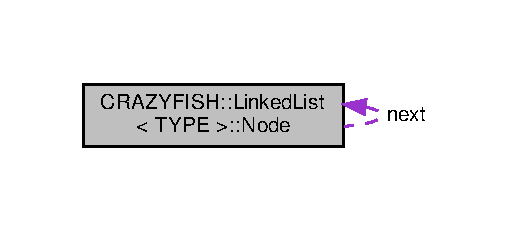
\includegraphics[width=245pt]{classCRAZYFISH_1_1LinkedList_1_1Node__coll__graph}
\end{center}
\end{figure}
\subsection*{Public Member Functions}
\begin{DoxyCompactItemize}
\item 
\hyperlink{classCRAZYFISH_1_1LinkedList_1_1Node_a05c9b60566f2abcb8449353d1efef015}{Node} ()
\item 
\hyperlink{classCRAZYFISH_1_1LinkedList_1_1Node_a8b39a874acc9d934134459cee3a1862b}{Node} (T\+Y\+PE \+\_\+d)
\item 
\hyperlink{classCRAZYFISH_1_1LinkedList_1_1Node_a7a19b881eef35ee20838dd763aa00a73}{$\sim$\+Node} ()
\end{DoxyCompactItemize}
\subsection*{Public Attributes}
\begin{DoxyCompactItemize}
\item 
T\+Y\+PE \hyperlink{classCRAZYFISH_1_1LinkedList_1_1Node_afe4cb216b2b093d60e522a69bfc575db}{value}
\item 
\hyperlink{classCRAZYFISH_1_1LinkedList_1_1Node}{Node} $\ast$ \hyperlink{classCRAZYFISH_1_1LinkedList_1_1Node_a3447e69abaf59c3c678fd370dd8f2f16}{next}
\end{DoxyCompactItemize}


\subsection{Detailed Description}
\subsubsection*{template$<$class T\+Y\+PE$>$\newline
class C\+R\+A\+Z\+Y\+F\+I\+S\+H\+::\+Linked\+List$<$ T\+Y\+P\+E $>$\+::\+Node}

A node of the linked List. 

\subsection{Constructor \& Destructor Documentation}
\mbox{\Hypertarget{classCRAZYFISH_1_1LinkedList_1_1Node_a05c9b60566f2abcb8449353d1efef015}\label{classCRAZYFISH_1_1LinkedList_1_1Node_a05c9b60566f2abcb8449353d1efef015}} 
\index{C\+R\+A\+Z\+Y\+F\+I\+S\+H\+::\+Linked\+List\+::\+Node@{C\+R\+A\+Z\+Y\+F\+I\+S\+H\+::\+Linked\+List\+::\+Node}!Node@{Node}}
\index{Node@{Node}!C\+R\+A\+Z\+Y\+F\+I\+S\+H\+::\+Linked\+List\+::\+Node@{C\+R\+A\+Z\+Y\+F\+I\+S\+H\+::\+Linked\+List\+::\+Node}}
\subsubsection{\texorpdfstring{Node()}{Node()}\hspace{0.1cm}{\footnotesize\ttfamily [1/2]}}
{\footnotesize\ttfamily template$<$class T\+Y\+PE$>$ \\
\hyperlink{classCRAZYFISH_1_1LinkedList}{C\+R\+A\+Z\+Y\+F\+I\+S\+H\+::\+Linked\+List}$<$ T\+Y\+PE $>$\+::Node\+::\+Node (\begin{DoxyParamCaption}{ }\end{DoxyParamCaption})\hspace{0.3cm}{\ttfamily [inline]}}

The default constructor. \mbox{\Hypertarget{classCRAZYFISH_1_1LinkedList_1_1Node_a8b39a874acc9d934134459cee3a1862b}\label{classCRAZYFISH_1_1LinkedList_1_1Node_a8b39a874acc9d934134459cee3a1862b}} 
\index{C\+R\+A\+Z\+Y\+F\+I\+S\+H\+::\+Linked\+List\+::\+Node@{C\+R\+A\+Z\+Y\+F\+I\+S\+H\+::\+Linked\+List\+::\+Node}!Node@{Node}}
\index{Node@{Node}!C\+R\+A\+Z\+Y\+F\+I\+S\+H\+::\+Linked\+List\+::\+Node@{C\+R\+A\+Z\+Y\+F\+I\+S\+H\+::\+Linked\+List\+::\+Node}}
\subsubsection{\texorpdfstring{Node()}{Node()}\hspace{0.1cm}{\footnotesize\ttfamily [2/2]}}
{\footnotesize\ttfamily template$<$class T\+Y\+PE$>$ \\
\hyperlink{classCRAZYFISH_1_1LinkedList}{C\+R\+A\+Z\+Y\+F\+I\+S\+H\+::\+Linked\+List}$<$ T\+Y\+PE $>$\+::Node\+::\+Node (\begin{DoxyParamCaption}\item[{T\+Y\+PE}]{\+\_\+d }\end{DoxyParamCaption})\hspace{0.3cm}{\ttfamily [inline]}}

Constructor, with the value is \+\_\+d.


\begin{DoxyParams}{Parameters}
{\em \+\_\+d} & The value to set. \\
\hline
\end{DoxyParams}
\mbox{\Hypertarget{classCRAZYFISH_1_1LinkedList_1_1Node_a7a19b881eef35ee20838dd763aa00a73}\label{classCRAZYFISH_1_1LinkedList_1_1Node_a7a19b881eef35ee20838dd763aa00a73}} 
\index{C\+R\+A\+Z\+Y\+F\+I\+S\+H\+::\+Linked\+List\+::\+Node@{C\+R\+A\+Z\+Y\+F\+I\+S\+H\+::\+Linked\+List\+::\+Node}!````~Node@{$\sim$\+Node}}
\index{````~Node@{$\sim$\+Node}!C\+R\+A\+Z\+Y\+F\+I\+S\+H\+::\+Linked\+List\+::\+Node@{C\+R\+A\+Z\+Y\+F\+I\+S\+H\+::\+Linked\+List\+::\+Node}}
\subsubsection{\texorpdfstring{$\sim$\+Node()}{~Node()}}
{\footnotesize\ttfamily template$<$class T\+Y\+PE$>$ \\
\hyperlink{classCRAZYFISH_1_1LinkedList}{C\+R\+A\+Z\+Y\+F\+I\+S\+H\+::\+Linked\+List}$<$ T\+Y\+PE $>$\+::Node\+::$\sim$\+Node (\begin{DoxyParamCaption}{ }\end{DoxyParamCaption})\hspace{0.3cm}{\ttfamily [inline]}}

The default destructor. 

\subsection{Member Data Documentation}
\mbox{\Hypertarget{classCRAZYFISH_1_1LinkedList_1_1Node_a3447e69abaf59c3c678fd370dd8f2f16}\label{classCRAZYFISH_1_1LinkedList_1_1Node_a3447e69abaf59c3c678fd370dd8f2f16}} 
\index{C\+R\+A\+Z\+Y\+F\+I\+S\+H\+::\+Linked\+List\+::\+Node@{C\+R\+A\+Z\+Y\+F\+I\+S\+H\+::\+Linked\+List\+::\+Node}!next@{next}}
\index{next@{next}!C\+R\+A\+Z\+Y\+F\+I\+S\+H\+::\+Linked\+List\+::\+Node@{C\+R\+A\+Z\+Y\+F\+I\+S\+H\+::\+Linked\+List\+::\+Node}}
\subsubsection{\texorpdfstring{next}{next}}
{\footnotesize\ttfamily template$<$class T\+Y\+PE$>$ \\
\hyperlink{classCRAZYFISH_1_1LinkedList_1_1Node}{Node}$\ast$ \hyperlink{classCRAZYFISH_1_1LinkedList}{C\+R\+A\+Z\+Y\+F\+I\+S\+H\+::\+Linked\+List}$<$ T\+Y\+PE $>$\+::Node\+::next}

The address of the next node of the linked List. \mbox{\Hypertarget{classCRAZYFISH_1_1LinkedList_1_1Node_afe4cb216b2b093d60e522a69bfc575db}\label{classCRAZYFISH_1_1LinkedList_1_1Node_afe4cb216b2b093d60e522a69bfc575db}} 
\index{C\+R\+A\+Z\+Y\+F\+I\+S\+H\+::\+Linked\+List\+::\+Node@{C\+R\+A\+Z\+Y\+F\+I\+S\+H\+::\+Linked\+List\+::\+Node}!value@{value}}
\index{value@{value}!C\+R\+A\+Z\+Y\+F\+I\+S\+H\+::\+Linked\+List\+::\+Node@{C\+R\+A\+Z\+Y\+F\+I\+S\+H\+::\+Linked\+List\+::\+Node}}
\subsubsection{\texorpdfstring{value}{value}}
{\footnotesize\ttfamily template$<$class T\+Y\+PE$>$ \\
T\+Y\+PE \hyperlink{classCRAZYFISH_1_1LinkedList}{C\+R\+A\+Z\+Y\+F\+I\+S\+H\+::\+Linked\+List}$<$ T\+Y\+PE $>$\+::Node\+::value}

The stored value. 

The documentation for this class was generated from the following file\+:\begin{DoxyCompactItemize}
\item 
\hyperlink{LinkedList_8h}{Linked\+List.\+h}\end{DoxyCompactItemize}

\chapter{File Documentation}
\hypertarget{LinkedList_8h}{}\section{Linked\+List.\+h File Reference}
\label{LinkedList_8h}\index{Linked\+List.\+h@{Linked\+List.\+h}}


An implementation of the dynamic A\+DT List. This is a demo for teaching, N\+OT recommended for any practical job.  


{\ttfamily \#include $<$iostream$>$}\newline
{\ttfamily \#include $<$limits$>$}\newline
{\ttfamily \#include $<$cstdlib$>$}\newline
Include dependency graph for Linked\+List.\+h\+:\nopagebreak
\begin{figure}[H]
\begin{center}
\leavevmode
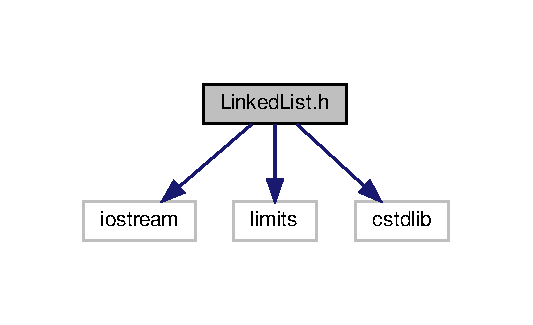
\includegraphics[width=256pt]{LinkedList_8h__incl}
\end{center}
\end{figure}
This graph shows which files directly or indirectly include this file\+:\nopagebreak
\begin{figure}[H]
\begin{center}
\leavevmode
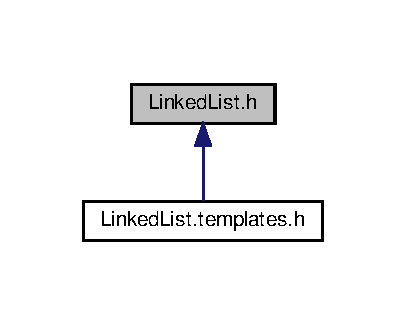
\includegraphics[width=195pt]{LinkedList_8h__dep__incl}
\end{center}
\end{figure}
\subsection*{Classes}
\begin{DoxyCompactItemize}
\item 
class \hyperlink{classCRAZYFISH_1_1LinkedList}{C\+R\+A\+Z\+Y\+F\+I\+S\+H\+::\+Linked\+List$<$ T\+Y\+P\+E $>$}
\item 
class \hyperlink{classCRAZYFISH_1_1LinkedList}{C\+R\+A\+Z\+Y\+F\+I\+S\+H\+::\+Linked\+List$<$ T\+Y\+P\+E $>$}
\item 
class \hyperlink{classCRAZYFISH_1_1LinkedList_1_1Node}{C\+R\+A\+Z\+Y\+F\+I\+S\+H\+::\+Linked\+List$<$ T\+Y\+P\+E $>$\+::\+Node}
\end{DoxyCompactItemize}
\subsection*{Functions}
\begin{DoxyCompactItemize}
\item 
template std\+::ostream \& {\bfseries C\+R\+A\+Z\+Y\+F\+I\+S\+H\+::operator$<$$<$} (std\+::ostream \&os, const Linked\+List$<$ T\+Y\+PE $>$ \&\+\_\+obj)
\end{DoxyCompactItemize}


\subsection{Detailed Description}
An implementation of the dynamic A\+DT List. This is a demo for teaching, N\+OT recommended for any practical job. 

\begin{DoxyAuthor}{Author}
Wang Heyu 
\end{DoxyAuthor}
\begin{DoxyDate}{Date}
Sat Aug 31 15\+:54\+:20 2019 
\end{DoxyDate}


\subsection{Function Documentation}
\mbox{\Hypertarget{LinkedList_8cpp_file_a0aecd881aa228dbbfef184d1201df0e5}\label{LinkedList_8cpp_file_a0aecd881aa228dbbfef184d1201df0e5}} 
\index{Linked\+List.\+h@{Linked\+List.\+h}!operator$<$$<$@{operator$<$$<$}}
\index{operator$<$$<$@{operator$<$$<$}!Linked\+List.\+h@{Linked\+List.\+h}}
\subsubsection{\texorpdfstring{operator$<$$<$()}{operator<<()}}
{\footnotesize\ttfamily std\+::ostream \& C\+R\+A\+Z\+Y\+F\+I\+S\+H\+::operator$<$$<$ (\begin{DoxyParamCaption}\item[{std\+::ostream \&}]{os,  }\item[{const \hyperlink{classCRAZYFISH_1_1LinkedList}{Linked\+List}$<$ T\+Y\+PE $>$ \&}]{\+\_\+obj }\end{DoxyParamCaption})}

To print out the content in streams.


\begin{DoxyParams}{Parameters}
{\em os} & an output stream followed. \\
\hline
{\em \+\_\+obj} & the List to output.\\
\hline
\end{DoxyParams}
\begin{DoxyReturn}{Returns}
the stream to output. 
\end{DoxyReturn}

%--- End generated contents ---

% Index
\backmatter
\newpage
\phantomsection
\clearemptydoublepage
\addcontentsline{toc}{chapter}{Index}
\printindex

\end{document}
